
\subsection{\label{sec:Tutorial-3d-hex8-static}Static Examples}

PyLith features discussed in this tutorial:
\begin{itemize}
\item Static solution
\item VTK output
\item Dirichlet displacement boundary conditions
\item Neumann traction boundary conditions
\item ZeroDispDB spatial database
\item SimpleDB spatial database
\item UniformDB spatial database
\item Static fault rupture
\item Specifying more than one material
\item Linearly elastic isotropic material
\end{itemize}

\subsubsection{Overview}

This set of examples describe the simplest class of problems for PyLith.
The problems are all purely elastic, and there is no time-dependence.
This set of elastostatic examples primarily demonstrates the application
of different types of boundary conditions in PyLith, as well as demonstrating
the use of a kinematic fault for a static problem. All of the examples
are contained in the directory \texttt{examples/3d/hex8}, and the
corresponding \texttt{.cfg} files are \texttt{step01.cfg}, \texttt{step02.cfg},
and \texttt{step03.cfg}. Each example may be run as follows:
\begin{lyxcode}
pylith~stepXX.cfg
\end{lyxcode}
This will cause PyLith to read the default parameters in \texttt{pylithapp.cfg},
and then override or augment them with the additional parameters in
the \texttt{stepXX.cfg} file. Each \texttt{.cfg} file is extensively
documented to provide detailed information on the various parameters.


\subsubsection{Step01 - Pure Dirichlet Boundary Conditions}

The \texttt{step01.cfg} file defines a problem with pure Dirichlet
(displacement) boundary conditions corresponding to compression in
the x-direction and shear in the y-direction. The bottom (minimum
z) boundary is held fixed in the z-direction. On the positive and
negative x-faces, compressional displacements of 1 m are applied in
the x-direction and shear displacements yielding a left-lateral sense
of shear are applied in the y-direction. In this example and in subsequent
examples we would like to output the displacement solution over a
subset of the domain corresponding to the ground surface. To do this,
we first set the output to an array of two output managers as follows:
\begin{lyxcode}
{[}pylithapp.timedependent.implicit{]}

\#~Set~the~output~to~an~array~of~2~output~managers.

\#~We~will~output~the~solution~over~the~domain~and~the~ground~surface.

output~=~{[}domain,subdomain{]}
\end{lyxcode}
We then define the subdomain output manager to correspond to a subset
of the domain:
\begin{lyxcode}
\#~Set~subdomain~component~to~OutputSolnSubset~(boundary~of~the~domain).

output.subdomain~=~pylith.meshio.OutputSolnSubset
\end{lyxcode}
Later (in the output section at the end of the file), we specify the
nodeset that corresponds to the desired output:
\begin{lyxcode}
\#~Give~basename~for~VTK~domain~output~of~solution~over~ground~surface.

{[}pylithapp.problem.formulation.output.subdomain{]}

\#~Name~of~nodeset~for~ground~surface.

label~=~face\_zpos

writer.filename~=~output/step01-groundsurf.vtk
\end{lyxcode}
For the boundary conditions, we must describe which degrees of freedom
are being constrained (\texttt{bc\_dof}), we must provide a the label
associated with the CUBIT nodeset associated with the BC, and we must
specify the type of spatial database is being used to describe the
boundary conditions. For the x-faces, we use a \texttt{SimpleDB} to
provide the displacements on the x-faces:
\begin{lyxcode}
\#~+x~face

{[}pylithapp.timedependent.bc.x\_pos{]}

bc\_dof~=~{[}0,~1{]}

label~=~face\_xpos

db\_initial~=~spatialdata.spatialdb.SimpleDB

db\_initial.label~=~Dirichlet~BC~on~+x

db\_initial.iohandler.filename~=~spatialdb/fixeddisp\_axial\_shear.spatialdb~\\
~\\


\#~-x~face

{[}pylithapp.timedependent.bc.x\_neg{]}

bc\_dof~=~{[}0,~1{]}

label~=~face\_xneg

db\_initial~=~spatialdata.spatialdb.SimpleDB

db\_initial.label~=~Dirichlet~BC~on~-x

db\_initial.iohandler.filename~=~spatialdb/fixeddisp\_axial\_shear.spatialdb
\end{lyxcode}
For a \texttt{SimpleDB}, we must provide a filename. The default spatial
database for \texttt{db\_initial} is \texttt{ZeroDispBC}, which automatically
applies zero displacements to all vertices in the nodeset, and no
filename is required (or needed). This is what we use for the bottom
of the mesh:
\begin{lyxcode}
\#~-z~face

{[}pylithapp.timedependent.bc.z\_neg{]}

bc\_dof~=~{[}2{]}

label~=~face\_zneg

db\_initial.label~=~Dirichlet~BC~on~-z
\end{lyxcode}
When we have run the simulation, the output VTK files will be contained
in \texttt{examples/3d/hex8/output} (all with a pvrefix of \texttt{step01}).
Results using ParaView are shown in Figure \vref{fig:step01-displ}.

\begin{figure}
\begin{centering}
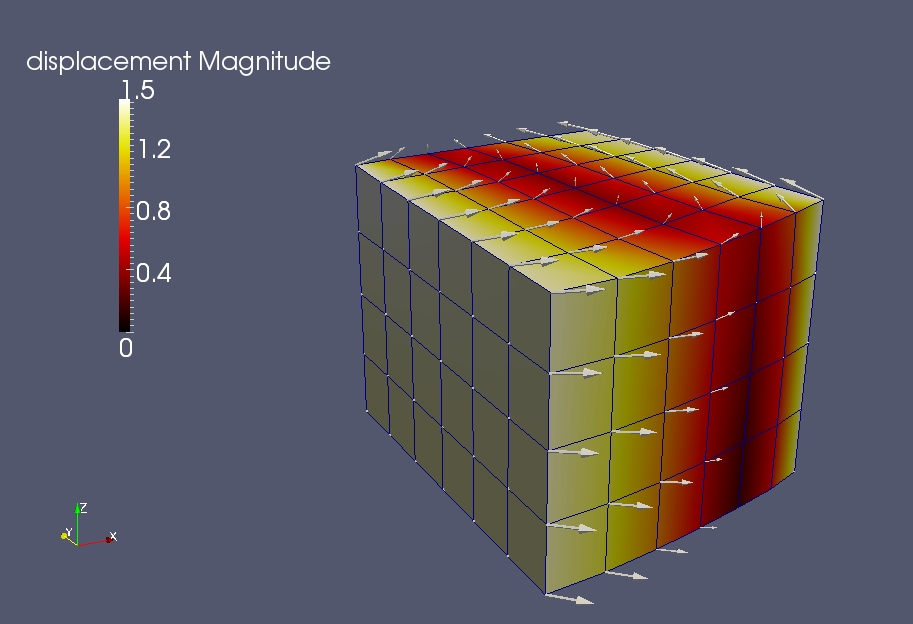
\includegraphics[width=10cm]{tutorials/3dhex8/figs/step01-displ}
\par\end{centering}

\caption{Displacement field for example step01 visualized using ParaView. The
mesh has been distorted by the computed displacements (magnified by
500), and the vectors show the computed displacements.\label{fig:step01-displ}}
\end{figure}



\subsubsection{Step02 - Dirichlet and Neumann Boundary Conditions}

The \texttt{step02.cfg} file defines a problem with Dirichlet (displacement)
boundary conditions corresponding to zero x and y-displacements applied
on the negative x-face and Neumann (traction) boundary conditions
corresponding to normal compression and horizontal shear applied on
the positive x-face. The bottom (negative z) boundary is held fixed
in the z-direction. The problem is similar to example step01, except
that 1 MPa of normal compression and 1 MPa of shear (in a left-lateral
sense) are applied on the positive x-face, and the negative x-face
is pinned in both the x and y-directions.

For the boundary conditions, we must first change the boundary condition
type for the positive x-face from the default Dirichlet to Neumann:
\begin{lyxcode}
\#~+x~face~-{}-~first~change~bc~type~to~Neumann

{[}pylithapp.timedependent.bc{]}

x\_pos~=~pylith.bc.Neumann~
\end{lyxcode}
We use a \texttt{SimpleDB} to describe the traction boundary conditions.
When applying traction boundary conditions over a surface, it is also
necessary to specify integration information for the surface. Since
this is a three-dimensional problem, the dimension of the surface
is 2. Since the cells being used are trilinear hexahedra, the cell
type is \texttt{FIATLagrange} and we use an integration order of 2.
A lower integration order would not provide sufficient accuracy while
a higher integration order would offer no benefit (while requiring
more computation time and storage):
\begin{lyxcode}
\#~+x~face

{[}pylithapp.timedependent.bc.x\_pos{]}

label~=~face\_xpos

db\_initial~=~spatialdata.spatialdb.SimpleDB

db\_initial.label~=~Neumann~BC~on~+x

db\_initial.iohandler.filename~=~spatialdb/tractions\_axial\_shear.spatialdb~\\
~\\


\#~We~must~specify~quadrature~information~for~the~cell~faces.

quadrature.cell~=~pylith.feassemble.FIATLagrange

quadrature.cell.dimension~=~2

quadrature.cell.quad\_order~=~2~
\end{lyxcode}
The boundary conditions on the negative x-face are simpler than they
were in example step01 (zero displacements in the x and y-directions),
so we can use the default \texttt{ZeroDispBC}:
\begin{lyxcode}
\#~-x~face

{[}pylithapp.timedependent.bc.x\_neg{]}

bc\_dof~=~{[}0,~1{]}~

label~=~face\_xneg

db\_initial.label~=~Dirichlet~BC~on~-x~
\end{lyxcode}
The boundary conditions on the negative z-face are supplied in the
same manner as for example step01. When we have run the simulation,
the output VTK files will be contained in \texttt{examples/3d/hex8/output}
(all with a pvrefix of \texttt{step02}). Results using ParaView are
shown in Figure \vref{fig:step02-displ}.
\begin{figure}
\centering{}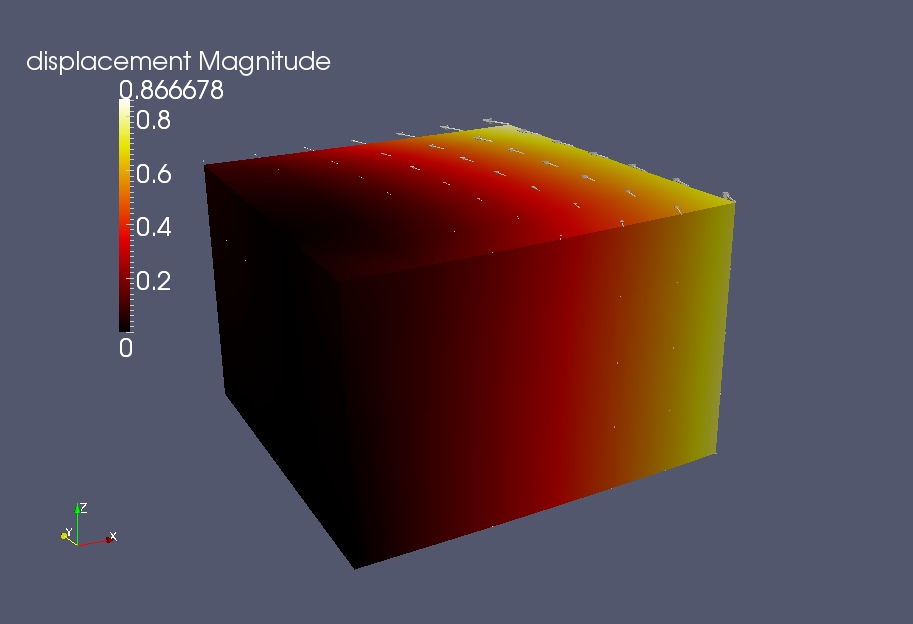
\includegraphics[width=10cm]{tutorials/3dhex8/figs/step02-displ}\caption{Displacement field for example step02 visualized using ParaView. The
mesh has been distorted by the computed displacements (magnified by
500), and the vectors show the computed displacements.\label{fig:step02-displ}.}
\end{figure}



\subsubsection{Step03 - Dirichlet Boundary Conditions with Kinematic Fault Slip}

The \texttt{step03.cfg} file describes a problem with Dirichlet (displacement)
boundary conditions corresponding to zero x and y-displacements applied
on the negative and positive x-faces and a vertical fault with a combination
of left-lateral and updip motion. The left-lateral component of fault
slip has a constant value of 2 m in the upper crust, and then decreases
linearly to zero at the base of the model. The reverse slip component
has a value of 0.25 m at the surface, and then decreases linearly
to zero at 2 km depth.

Due to the simplicity of the boundary conditions, we are able to use
the default \texttt{ZeroDispBC} for the positive and negative x-faces,
as well as the negative z-face. To use a fault, we must first define
a fault interface. We do this by providing an array containing a single
interface:
\begin{lyxcode}
{[}pylithapp.timedependent{]}

\#~Set~interfaces~to~an~array~of~1~fault:~'fault'.

interfaces~=~{[}fault{]}~
\end{lyxcode}
For this example we specify the fault slip, so we set the interface
type to \texttt{FaultCohesiveKin}:
\begin{lyxcode}
\#~Set~the~type~of~fault~interface~condition.

{[}pylithapp.timedependent.interfaces{]}

fault~=~pylith.faults.FaultCohesiveKin~
\end{lyxcode}
We must then identify the nodeset corresponding to the fault, and
provide integration information for the fault surface:
\begin{lyxcode}
\#~Set~the~parameters~for~the~fault~interface~condition.

{[}pylithapp.timedependent.interfaces.fault{]}

\#~The~label~corresponds~to~the~name~of~the~nodeset~in~CUBIT.

label~=~fault~\\
~\\


\#~We~must~define~the~quadrature~information~for~fault~cells.

\#~The~fault~cells~are~2D~(surface).

quadrature.cell~=~pylith.feassemble.FIATLagrange

quadrature.cell.dimension~=~2~
\end{lyxcode}
We retain the default \texttt{StepSlipFn} since we want static fault
slip. Finally, we use one \texttt{SimpleDB} to define the spatial
variation of fault slip, and another \texttt{SimpleDB} to define the
spatial variation in slip initiation times (the start time is 0.0
everywhere since this is a static problem):
\begin{lyxcode}
\#~The~slip~time~and~final~slip~are~defined~in~spatial~databases.~\\
{[}pylithapp.timedependent.interfaces.fault.eq\_srcs.rupture.slip\_function{]}~\\
slip.iohandler.filename~=~spatialdb/finalslip.spatialdb

slip.query\_type~=~linear

slip\_time.iohandler.filename~=~spatialdb/sliptime.spatialdb~
\end{lyxcode}
Since the problem now contains a fault, we can request that fault
infomation is also output:
\begin{lyxcode}
\#~Give~basename~for~VTK~fault~output.

{[}pylithapp.problem.interfaces.fault.output{]}

writer.filename~=~output/step03-fault.vtk~
\end{lyxcode}
This will result in two extra files being produced. The first file
(\texttt{step03-fault\_info.vtk}) contains information such as the
normal directions to the fault surface, the applied fault slip, and
the fault slip times. The second file (\texttt{step03-fault\_t0000000.vtk})
contains the cumulative fault slip for the time step and the change
in tractions on the fault surface due to the slip. When we have run
the simulation, the output VTK files will be contained in \texttt{examples/3d/hex8/output}
(all with a pvrefix of \texttt{step03}). Results using ParaView are
shown in Figure \vref{fig:step03-displ}.
\begin{figure}
\centering{}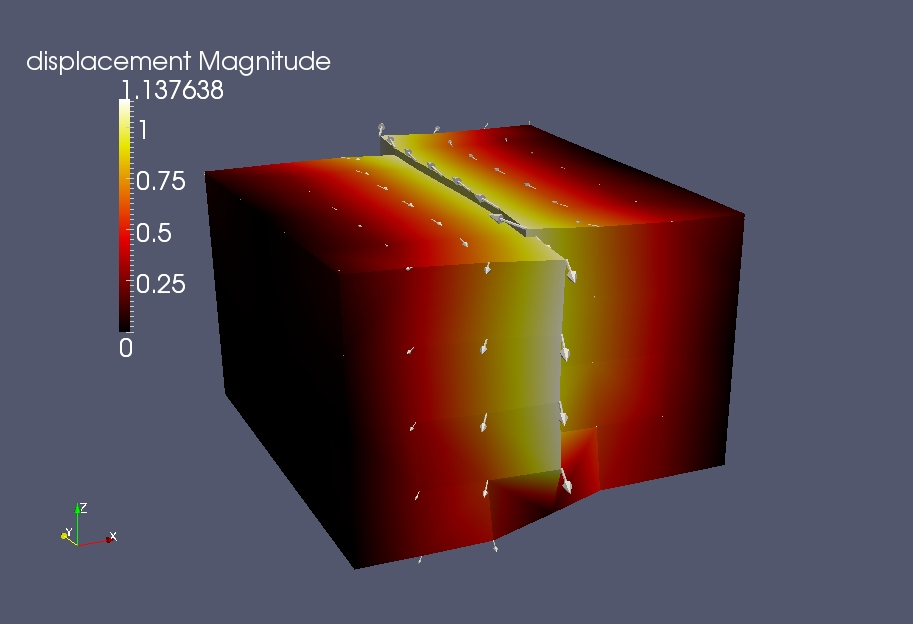
\includegraphics[width=10cm]{tutorials/3dhex8/figs/step03-displ}\caption{Displacement field for example step03 visualized using ParaView. The
mesh has been distorted by the computed displacements (magnified by
500), and the vectors show the computed displacements.\label{fig:step03-displ}.}
\end{figure}

